\documentclass[aspectratio=169]{beamer}

%\documentclass[handout]{beamer}
%% To make 4 per page
%\usepackage{pgfpages}
%\mode<handout>{\setbeamercolor{background canvas}{bg=white}}
%\pgfpagesuselayout{4 on 1}[letterpaper,landscape]%,border shrink=5mm]

\usetheme{default}
% Slide setup, colour independent

\usepackage{amsmath,amssymb,amsthm}
\usepackage{colortbl}
\usepackage{bm}
\usepackage{xcolor}
\usepackage{dsfont}
\usepackage{setspace}
%\usepackage{subfigure}
% To use \ding{234} and the like
\usepackage{pifont}
% To cross reference between slide files
\usepackage{zref-xr,zref-user}
% Use something like
% \zexternaldocument{fileI}
% in the tex files. And cite using \zref instead of \ref

% Fields and the like
\def\IC{\mathbb{C}}
\def\IF{\mathbb{F}}
\def\II{\mathbb{I}}
\def\IJ{\mathbb{J}}
\def\IM{\mathbb{M}}
\def\IN{\mathbb{N}}
\def\IP{\mathbb{P}}
\def\IR{\mathbb{R}}
\def\IZ{\mathbb{Z}}
\def\11{\mathds{1}}


% Bold lowercase
\def\ba{\mathbf{a}}
\def\bb{\mathbf{b}}
\def\bc{\mathbf{c}}
\def\bd{\mathbf{d}}
\def\be{\mathbf{e}}
\def\bf{\mathbf{f}}
\def\bh{\mathbf{h}}
\def\bi{\mathbf{i}}
\def\bj{\mathbf{j}}
\def\bk{\mathbf{k}}
\def\bn{\mathbf{n}}
\def\bp{\mathbf{p}}
\def\br{\mathbf{r}}
\def\bs{\mathbf{s}}
\def\bu{\mathbf{u}}
\def\bv{\mathbf{v}}
\def\bw{\mathbf{w}}
\def\bx{\mathbf{x}}
\def\by{\mathbf{y}}
\def\bz{\mathbf{z}}

% Bold capitals
\def\bB{\mathbf{B}}
\def\bD{\mathbf{D}}
\def\bF{\mathbf{F}}
\def\bG{\mathbf{G}}
\def\bI{\mathbf{I}}
\def\bL{\mathbf{L}}
\def\bN{\mathbf{N}}
\def\bP{\mathbf{P}}
\def\bR{\mathbf{R}}
\def\bS{\mathbf{S}}
\def\bT{\mathbf{T}}
\def\bX{\mathbf{X}}

% Bold numbers
\def\b0{\mathbf{0}}

% Bold greek
\bmdefine{\bmu}{\bm{\mu}}
\def\bphi{\bm{\phi}}
\def\bvarphi{\bm{\varphi}}

% Bold red sentence
\def\boldred#1{{\color{red}\textbf{#1}}}
\def\defword#1{{\color{orange}\textbf{#1}}}

% Caligraphic letters
\def\A{\mathcal{A}}
\def\B{\mathcal{B}}
\def\C{\mathcal{C}}
\def\D{\mathcal{D}}
\def\E{\mathcal{E}}
\def\F{\mathcal{F}}
\def\G{\mathcal{G}}
\def\H{\mathcal{H}}
\def\I{\mathcal{I}}
\def\L{\mathcal{L}}
\def\M{\mathcal{M}}
\def\N{\mathcal{N}}
\def\P{\mathcal{P}}
\def\R{\mathcal{R}}
\def\S{\mathcal{S}}
\def\T{\mathcal{T}}
\def\U{\mathcal{U}}
\def\V{\mathcal{V}}

% tt font for code
\def\code#1{{\tt #1}}

% i.e., e.g.
\def\eg{\emph{e.g.}}
\def\ie{\emph{i.e.}}


% Operators and special symbols
\def\nbOne{{\mathchoice {\rm 1\mskip-4mu l} {\rm 1\mskip-4mu l}
{\rm 1\mskip-4.5mu l} {\rm 1\mskip-5mu l}}}
\def\cov{\ensuremath{\mathsf{cov}}}
\def\Var{\ensuremath{\mathsf{Var}\ }}
\def\Im{\textrm{Im}\;}
\def\Re{\textrm{Re}\;}
\def\det{\ensuremath{\mathsf{det}}}
\def\diag{\ensuremath{\mathsf{diag}}}
\def\nullspace{\ensuremath{\mathsf{null}}}
\def\nullity{\ensuremath{\mathsf{nullity}}}
\def\rank{\ensuremath{\mathsf{rank}}}
\def\range{\ensuremath{\mathsf{range}}}
\def\sgn{\ensuremath{\mathsf{sgn}}}
\def\Span{\ensuremath{\mathsf{span}}}
\def\tr{\ensuremath{\mathsf{tr}}}
\def\imply{$\Rightarrow$}
\def\restrictTo#1#2{\left.#1\right|_{#2}}
\newcommand{\parallelsum}{\mathbin{\!/\mkern-5mu/\!}}
\def\dsum{\mathop{\displaystyle \sum }}%
\def\dind#1#2{_{\substack{#1\\ #2}}}

\DeclareMathOperator{\GL}{GL}
\DeclareMathOperator{\Rel}{Re}
\def\Nt#1{\left|\!\left|\!\left|#1\right|\!\right|\!\right|}
\newcommand{\tripbar}{|\! |\! |}



% The beamer bullet (in base colour)
\def\bbullet{\leavevmode\usebeamertemplate{itemize item}\ }

% Theorems and the like
\newtheorem{proposition}[theorem]{Proposition}
\newtheorem{property}[theorem]{Property}
\newtheorem{importantproperty}[theorem]{Property}
\newtheorem{importanttheorem}[theorem]{Theorem}
%\newtheorem{lemma}[theorem]{Lemma}
%\newtheorem{corollary}[theorem]{Corollary}
\newtheorem{remark}[theorem]{Remark}
\setbeamertemplate{theorems}[numbered]
%\setbeamertemplate{theorems}[ams style]

%
%\usecolortheme{orchid}
%\usecolortheme{orchid}

\def\red{\color[rgb]{1,0,0}}
\def\blue{\color[rgb]{0,0,1}}
\def\green{\color[rgb]{0,1,0}}


% Get rid of navigation stuff
\setbeamertemplate{navigation symbols}{}

% Set footline/header line
\setbeamertemplate{footline}
{%
\quad p. \insertpagenumber \quad--\quad \insertsection\vskip2pt
}
% \setbeamertemplate{headline}
% {%
% \quad\insertsection\hfill p. \insertpagenumber\quad\mbox{}\vskip2pt
% }


\makeatletter
\newlength\beamerleftmargin
\setlength\beamerleftmargin{\Gm@lmargin}
\makeatother

% Colours for special pages
\def\extraContent{yellow!20}


%%%%%%%%%%%%%%%%%
\usepackage{tikz}
\usetikzlibrary{shapes,arrows}
\usetikzlibrary{positioning}
\usetikzlibrary{shapes.symbols,shapes.callouts,patterns}
\usetikzlibrary{calc,fit}
\usetikzlibrary{backgrounds}
\usetikzlibrary{decorations.pathmorphing,fit,petri}
\usetikzlibrary{automata}
\usetikzlibrary{fadings}
\usetikzlibrary{patterns,hobby}

\usetikzlibrary{backgrounds,fit,petri}


\usepackage{pgfplots}
\pgfplotsset{compat=1.6}
\pgfplotsset{ticks=none}

\usetikzlibrary{decorations.markings}
\usetikzlibrary{arrows.meta}
\tikzset{>=stealth}

% For tikz
\usetikzlibrary{shapes,arrows}
\usetikzlibrary{positioning}
\tikzstyle{cloud} = [draw, ellipse,fill=red!20, node distance=0.87cm,
minimum height=2em]
\tikzstyle{line} = [draw, -latex']


%%% For max frame images
\newenvironment{changemargin}[2]{%
\begin{list}{}{%
\setlength{\topsep}{0pt}%
\setlength{\leftmargin}{#1}%
\setlength{\rightmargin}{#2}%
\setlength{\listparindent}{\parindent}%
\setlength{\itemindent}{\parindent}%
\setlength{\parsep}{\parskip}%
}%
\item[]}{\end{list}}


% Make one image take up the entire slide content area in beamer,.:
% centered/centred full-screen image, with title:
% This uses the whole screen except for the 1cm border around it
% all. 128x96mm
\newcommand{\titledFrameImage}[2]{
\begin{frame}{#1}
%\begin{changemargin}{-1cm}{-1cm}
\begin{center}
\includegraphics[width=108mm,height=\textheight,keepaspectratio]{#2}
\end{center}
%\end{changemargin}
\end{frame}
}

% Make one image take up the entire slide content area in beamer.:
% centered/centred full-screen image, no title:
% This uses the whole screen except for the 1cm border around it
% all. 128x96mm
\newcommand{\plainFrameImage}[1]{
\begin{frame}[plain]
%\begin{changemargin}{-1cm}{-1cm}
\begin{center}
\includegraphics[width=108mm,height=76mm,keepaspectratio]{#1}
\end{center}
%\end{changemargin}
\end{frame}
}

% Make one image take up the entire slide area, including borders, in beamer.:
% centered/centred full-screen image, no title:
% This uses the entire whole screen
\newcommand{\maxFrameImage}[1]{
\begin{frame}[plain]
\begin{changemargin}{-1cm}{-1cm}
\begin{center}
\includegraphics[width=\paperwidth,height=\paperheight,keepaspectratio]
{#1}
\end{center}
\end{changemargin}
\end{frame}
}

% This uses the entire whole screen (to include in frame)
\newcommand{\maxFrameImageNoFrame}[1]{
\begin{changemargin}{-1cm}{-1cm}
\begin{center}
\includegraphics[width=\paperwidth,height=0.99\paperheight,keepaspectratio]
{#1}
\end{center}
\end{changemargin}
}

% Make one image take up the entire slide area, including borders, in beamer.:
% centered/centred full-screen image, no title:
% This uses the entire whole screen
\newcommand{\maxFrameImageColor}[2]{
\begin{frame}[plain]
\setbeamercolor{normal text}{bg=#2!20}
\begin{changemargin}{-1cm}{-1cm}
\begin{center}
\includegraphics[width=\paperwidth,height=\paperheight,keepaspectratio]
{#1}
\end{center}
\end{changemargin}
\end{frame}
}


\usepackage{tikz}
\usetikzlibrary{patterns,hobby}
\usepackage{pgfplots}
\pgfplotsset{compat=1.6}
\pgfplotsset{ticks=none}

\usetikzlibrary{backgrounds}
\usetikzlibrary{decorations.markings}
\usetikzlibrary{arrows.meta}
\tikzset{>=stealth}

\tikzset{
  clockwise arrows/.style={
    postaction={
      decorate,
      decoration={
        markings,
        mark=between positions 0.1 and 0.9 step 40pt with {\arrow{>}},
   }}}}


   %%%%%%%%%%%
% To have links to parts in the outline
\makeatletter
\AtBeginPart{%
  \addtocontents{toc}{\protect\beamer@partintoc{\the\c@part}{\beamer@partnameshort}{\the\c@page}}%
}
%% number, shortname, page.
\providecommand\beamer@partintoc[3]{%
  \ifnum\c@tocdepth=-1\relax
    % requesting onlyparts.
    \makebox[6em]{Part #1:} \textcolor{green!30!blue}{\hyperlink{#2}{#2}}
    \par
  \fi
}
\define@key{beamertoc}{onlyparts}[]{%
  \c@tocdepth=-1\relax
}
\makeatother%

\newcommand{\nameofthepart}{}
\newcommand{\nupart}[1]%
    {   \part{#1}%
        \renewcommand{\nameofthepart}{#1}%
        {
          \setbeamercolor{background canvas}{bg=orange!50}
          \begin{frame}{#1}%\partpage 
          \hypertarget{\nameofthepart}{}\tableofcontents%
          \end{frame}
        }
    }



\usecolortheme{orchid}

%% Listings
\usepackage{listings}
\definecolor{mygreen}{rgb}{0,0.6,0}
\definecolor{mygray}{rgb}{0.5,0.5,0.5}
\definecolor{mymauve}{rgb}{0.58,0,0.82}
\definecolor{mygold}{rgb}{1,0.843,0}
\definecolor{myblue}{rgb}{0.537,0.812,0.941}

\definecolor{lgreen}{rgb}{0.6,0.9,.6}
\definecolor{lred}{rgb}{1,0.5,.5}

\lstloadlanguages{R}
\lstset{ %
  language=R,
  backgroundcolor=\color{black!05},   % choose the background color
  basicstyle=\footnotesize\ttfamily,        % size of fonts used for the code
  breaklines=true,                 % automatic line breaking only at whitespace
  captionpos=b,                    % sets the caption-position to bottom
  commentstyle=\color{mygreen},    % comment style
  escapeinside={\%*}{*)},          % if you want to add LaTeX within your code
  keywordstyle=\color{red},       % keyword style
  stringstyle=\color{mygold},     % string literal style
  keepspaces=true,
  columns=fullflexible,
  tabsize=4,
}
% Could also do (in lstset)
% basicstyle==\fontfamily{pcr}\footnotesize
\lstdefinelanguage{Renhanced}%
  {keywords={abbreviate,abline,abs,acos,acosh,action,add1,add,%
      aggregate,alias,Alias,alist,all,anova,any,aov,aperm,append,apply,%
      approx,approxfun,apropos,Arg,args,array,arrows,as,asin,asinh,%
      atan,atan2,atanh,attach,attr,attributes,autoload,autoloader,ave,%
      axis,backsolve,barplot,basename,besselI,besselJ,besselK,besselY,%
      beta,binomial,body,box,boxplot,break,browser,bug,builtins,bxp,by,%
      c,C,call,Call,case,cat,category,cbind,ceiling,character,char,%
      charmatch,check,chol,chol2inv,choose,chull,class,close,cm,codes,%
      coef,coefficients,co,col,colnames,colors,colours,commandArgs,%
      comment,complete,complex,conflicts,Conj,contents,contour,%
      contrasts,contr,control,helmert,contrib,convolve,cooks,coords,%
      distance,coplot,cor,cos,cosh,count,fields,cov,covratio,wt,CRAN,%
      create,crossprod,cummax,cummin,cumprod,cumsum,curve,cut,cycle,D,%
      data,dataentry,date,dbeta,dbinom,dcauchy,dchisq,de,debug,%
      debugger,Defunct,default,delay,delete,deltat,demo,de,density,%
      deparse,dependencies,Deprecated,deriv,description,detach,%
      dev2bitmap,dev,cur,deviance,off,prev,,dexp,df,dfbetas,dffits,%
      dgamma,dgeom,dget,dhyper,diag,diff,digamma,dim,dimnames,dir,%
      dirname,dlnorm,dlogis,dnbinom,dnchisq,dnorm,do,dotplot,double,%
      download,dpois,dput,drop,drop1,dsignrank,dt,dummy,dump,dunif,%
      duplicated,dweibull,dwilcox,dyn,edit,eff,effects,eigen,else,%
      emacs,end,environment,env,erase,eval,equal,evalq,example,exists,%
      exit,exp,expand,expression,External,extract,extractAIC,factor,%
      fail,family,fft,file,filled,find,fitted,fivenum,fix,floor,for,%
      For,formals,format,formatC,formula,Fortran,forwardsolve,frame,%
      frequency,ftable,ftable2table,function,gamma,Gamma,gammaCody,%
      gaussian,gc,gcinfo,gctorture,get,getenv,geterrmessage,getOption,%
      getwd,gl,glm,globalenv,gnome,GNOME,graphics,gray,grep,grey,grid,%
      gsub,hasTsp,hat,heat,help,hist,home,hsv,httpclient,I,identify,if,%
      ifelse,Im,image,\%in\%,index,influence,measures,inherits,install,%
      installed,integer,interaction,interactive,Internal,intersect,%
      inverse,invisible,IQR,is,jitter,kappa,kronecker,labels,lapply,%
      layout,lbeta,lchoose,lcm,legend,length,levels,lgamma,library,%
      licence,license,lines,list,lm,load,local,locator,log,log10,log1p,%
      log2,logical,loglin,lower,lowess,ls,lsfit,lsf,ls,machine,Machine,%
      mad,mahalanobis,make,link,margin,match,Math,matlines,mat,matplot,%
      matpoints,matrix,max,mean,median,memory,menu,merge,methods,min,%
      missing,Mod,mode,model,response,mosaicplot,mtext,mvfft,na,nan,%
      names,omit,nargs,nchar,ncol,NCOL,new,next,NextMethod,nextn,%
      nlevels,nlm,noquote,NotYetImplemented,NotYetUsed,nrow,NROW,null,%
      numeric,\%o\%,objects,offset,old,on,Ops,optim,optimise,optimize,%
      options,or,order,ordered,outer,package,packages,page,pairlist,%
      pairs,palette,panel,par,parent,parse,paste,path,pbeta,pbinom,%
      pcauchy,pchisq,pentagamma,persp,pexp,pf,pgamma,pgeom,phyper,pico,%
      pictex,piechart,Platform,plnorm,plogis,plot,pmatch,pmax,pmin,%
      pnbinom,pnchisq,pnorm,points,poisson,poly,polygon,polyroot,pos,%
      postscript,power,ppoints,ppois,predict,preplot,pretty,Primitive,%
      print,prmatrix,proc,prod,profile,proj,prompt,prop,provide,%
      psignrank,ps,pt,ptukey,punif,pweibull,pwilcox,q,qbeta,qbinom,%
      qcauchy,qchisq,qexp,qf,qgamma,qgeom,qhyper,qlnorm,qlogis,qnbinom,%
      qnchisq,qnorm,qpois,qqline,qqnorm,qqplot,qr,Q,qty,qy,qsignrank,%
      qt,qtukey,quantile,quasi,quit,qunif,quote,qweibull,qwilcox,%
      rainbow,range,rank,rbeta,rbind,rbinom,rcauchy,rchisq,Re,read,csv,%
      csv2,fwf,readline,socket,real,Recall,rect,reformulate,regexpr,%
      relevel,remove,rep,repeat,replace,replications,report,require,%
      resid,residuals,restart,return,rev,rexp,rf,rgamma,rgb,rgeom,R,%
      rhyper,rle,rlnorm,rlogis,rm,rnbinom,RNGkind,rnorm,round,row,%
      rownames,rowsum,rpois,rsignrank,rstandard,rstudent,rt,rug,runif,%
      rweibull,rwilcox,sample,sapply,save,scale,scan,scan,screen,sd,se,%
      search,searchpaths,segments,seq,sequence,setdiff,setequal,set,%
      setwd,show,sign,signif,sin,single,sinh,sink,solve,sort,source,%
      spline,splinefun,split,sqrt,stars,start,stat,stem,step,stop,%
      storage,strstrheight,stripplot,strsplit,structure,strwidth,sub,%
      subset,substitute,substr,substring,sum,summary,sunflowerplot,svd,%
      sweep,switch,symbol,symbols,symnum,sys,status,system,t,table,%
      tabulate,tan,tanh,tapply,tempfile,terms,terrain,tetragamma,text,%
      time,title,topo,trace,traceback,transform,tri,trigamma,trunc,try,%
      ts,tsp,typeof,unclass,undebug,undoc,union,unique,uniroot,unix,%
      unlink,unlist,unname,untrace,update,upper,url,UseMethod,var,%
      variable,vector,Version,vi,warning,warnings,weighted,weights,%
      which,while,window,write,\%x\%,x11,X11,xedit,xemacs,xinch,xor,%
      xpdrows,xy,xyinch,yinch,zapsmall,zip},%
   otherkeywords={!,!=,~,$,*,\%,\&,\%/\%,\%*\%,\%\%,<-,<<-,_,/},%
   alsoother={._$},%
   sensitive,%
   morecomment=[l]\#,%
   morestring=[d]",%
   morestring=[d]'% 2001 Robert Denham
  }%

%%%%%%% 
%% Definitions in yellow boxes
\usepackage{etoolbox}
\setbeamercolor{block title}{use=structure,fg=structure.fg,bg=structure.fg!40!bg}
\setbeamercolor{block body}{parent=normal text,use=block title,bg=block title.bg!20!bg}

\BeforeBeginEnvironment{definition}{%
	\setbeamercolor{block title}{fg=black,bg=yellow!20!white}
	\setbeamercolor{block body}{fg=black, bg=yellow!05!white}
}
\AfterEndEnvironment{definition}{
	\setbeamercolor{block title}{use=structure,fg=structure.fg,bg=structure.fg!20!bg}
	\setbeamercolor{block body}{parent=normal text,use=block title,bg=block title.bg!50!bg, fg=black}
}
\BeforeBeginEnvironment{importanttheorem}{%
	\setbeamercolor{block title}{fg=black,bg=red!20!white}
	\setbeamercolor{block body}{fg=black, bg=red!05!white}
}
\AfterEndEnvironment{importanttheorem}{
	\setbeamercolor{block title}{use=structure,fg=structure.fg,bg=structure.fg!20!bg}
	\setbeamercolor{block body}{parent=normal text,use=block title,bg=block title.bg!50!bg, fg=black}
}
\BeforeBeginEnvironment{importantproperty}{%
	\setbeamercolor{block title}{fg=black,bg=red!50!white}
	\setbeamercolor{block body}{fg=black, bg=red!30!white}
}
\AfterEndEnvironment{importantproperty}{
	\setbeamercolor{block title}{use=structure,fg=structure.fg,bg=structure.fg!20!bg}
	\setbeamercolor{block body}{parent=normal text,use=block title,bg=block title.bg!50!bg, fg=black}
}


% Beginning of a section
\AtBeginSection[]{
	{
		\setbeamercolor{background canvas}{bg=yellow!10}
		\begin{frame}[noframenumbering,plain]
			\framesubtitle{\nameofthepart Chapter \insertromanpartnumber \ -- \iteminsert{\insertpart}}
			\tableofcontents[
				currentsection,
				sectionstyle=show/shaded,
				subsectionstyle=show/show/hide]
		\end{frame}
	\addtocounter{page}{-1}
	%\addtocounter{framenumber}{-1} 
	}
}

% Beginning of a section
\AtBeginSubsection[]{
	{
		\setbeamercolor{background canvas}{bg=green!10}
		\begin{frame}[noframenumbering,plain]
				\framesubtitle{\nameofthepart Chapter \insertromanpartnumber \ -- \iteminsert{\insertpart}}
				\tableofcontents[
					currentsection,
					sectionstyle=show/show,
					currentsubsection,
					subsectionstyle=show/shaded/hide]
			\end{frame}
		\addtocounter{page}{-1}
	}
}

% To cross reference from other slide files
\zexternaldocument{MATH-4370-7370-slides-03-eigenpairs-similarity}
\zexternaldocument{MATH-4370-7370-slides-06-nonnegative-matrices}

% To have theorems and everything derived prefixed by the slide set
% number
\renewcommand{\thetheorem}{7.\arabic{theorem}}

\title{Essentially nonnegative matrices and M-matrices}
\author{Julien Arino}
\date{Fall 2023}

%%%%%%%%%%%%%%%%%%%%%
%%%%%%%%%%%%%%%%%%%%%
%%%%%%%%%%%%%%%%%%%%%
%%%%%%%%%%%%%%%%%%%%%
%%%%%%%%%%%%%%%%%%%%%
%%%%%%%%%%%%%%%%%%%%%
%%%%%%%%%%%%%%%%%%%%%
%%%%%%%%%%%%%%%%%%%%%
\begin{document}

% The title page
\begin{frame}[noframenumbering,plain]
  \begin{tikzpicture}[remember picture,overlay]
    \node[above right,inner sep=0pt] at (current page.south west)
    {
        
\includegraphics[width=\paperwidth]{title-page-picture.png}
    };
\end{tikzpicture}
	\titlepage
\end{frame}
\addtocounter{page}{-1}
  
  
\begin{frame}{Outline}
	  \tableofcontents[hideallsubsections]
\end{frame}
\addtocounter{page}{-1}


%%%%%%%%%%%%%%%%%%%%%%%%%%%
%%%%%%%%%%%%%%%%%%%%%%%%%%%
%%%%%%%%%%%%%%%%%%%%%%%%%%%
%%%%%%%%%%%%%%%%%%%%%%%%%%%
\section{Essentially nonnegative matrices}

\begin{frame}
The Perron-Frobenius can be applied not only to nonnegative matrices, but also to matrices that are \emph{essentially nonnegative}, in the sense that they are nonnegative except perhaps along the main diagonal
\vfill
\begin{definition}
A matrix $A\in \M_n$ is \defword{essentially nonegative}\index{matrix!essentially nonegative} (or \defword{quasi-positive}\index{matrix!quasi-positive}) if there exist $\alpha \in \IR$ such that $A+\alpha \mathbb{I}\geq 0$
\end{definition}
\vfill
\begin{remark}
    An essentially nonnegative matrix $A$ has non-negative off-diagonal entries. The sign of the diagonal entries is not relevant
\end{remark}
\end{frame}


\begin{frame}
\begin{remark}
Irreducibility of a matrix is not affected by the nature of its diagonal entries.  Indeed, consider an essentially nonnegative matrix $A$. The existence of a directed path in $G(A)$ does not depend on the existence of ``self-loops''. The same is not true of \emph{primitive} matrices, where the presence of negative entries on the main diagonal has an influence on the values of $A^k$ and thus ultimately, on the capacity to find $k$ such that $A^k>0$
\end{remark}
\end{frame}


\begin{frame}
So we can apply the ``weak'' versions of the Perron-Frobenius Theorem (the imprimitive cases in Theorem~\zref{th:PF_allCases}) to $A+\alpha \mathbb{I}$, which is a nonnegative matrix (potentially irreducible). One important ingredient is a result that was proved as Theorem~\ref{th:spectrum_shift}. Namely, that perturbations of the entire diagonal by the same scalar lead to a shift of the spectrum; this is summarised as
\[
\sigma(A+\alpha \mathbb{I})=\{ \lambda_1+\alpha, \dots, \lambda_n+\alpha,\quad \lambda_i\in \sigma(A)\}
\]
\end{frame}



\begin{frame}
\begin{definition}[Spectral abscissa]
Let $A\in \M_n$. The \defword{spectral abscissa} of $A$, $s(A)$, is 
\[
s(A)= \max\{\Rel(\lambda), \lambda\in \sigma(A)\}
\]
\end{definition}
\vfill
\begin{theorem}\label{th:PF_essentially_nonneg}
Let $A\in\M_n(\IR)$ be essentially nonnegative. Then $s(A)$ is an eigenvalue of $A$ and is associated to a nonnegative eigenvector. If, additionally, $A$ is irreducible, then $s(A)$ is simple and is associated to a positive eigenvector
\end{theorem}
\end{frame}



%%%%%%%%%%%%%%%%%%%%%%%
%%%%%%%%%%%%%%%%%%%%%%%
%%%%%%%%%%%%%%%%%%%%%%%
%%%%%%%%%%%%%%%%%%%%%%%
\section{Z-matrices}
\label{sec:Z_matrices}

\begin{frame}
\begin{definition}
A matrix is of class $Z_n$ if it is in $\M_n(\IR)$ and such that $a_{i,j}\leq 0$, $i \neq j$, $i,j=1,\ldots,n$
\[
    Z_n=\{A\in \M_n: a_{i,j}\leq 0, i\neq j\}
\]
We also say that $A\in Z_n$ has the \defword{$Z$-sign pattern}
\end{definition}
\end{frame}


\begin{frame}
\begin{theorem}[\cite{Fiedler2008}]
Let $A\in Z_n$. TFAE
\begin{enumerate}
    \item There is a nonnegative vector $x$ such that $Ax>0$
    \item There is a positive vector $x$ such that $Ax>0$
    \item There is a diagonal matrix $\diag(D)>0$ such that the entries in $AD=[w_{ik}]$ are such that 
    \[w_{ii}> \sum\limits_{k\neq i} | w_{ik}| \forall i\]
    \item For any $B\in Z_n$ such that $A\geq A$, then $B$ is nonsingular 
    \item Every real eigenvalue of any principal submatrix of $A$ is positive.
    \item All principal minors of $A$ are positive
\end{enumerate}
\end{theorem}
\end{frame}

\begin{frame}
\addtocounter{theorem}{-1}
\begin{theorem}[Continued]
\begin{enumerate}
    \setcounter{enumi}{6}
    \item For all $k= 1, \dots, n$, the sum of all principal minors is positive
    \item Every real eigenvalue of $A$ is positive
    \item There exists a matrix $C\geq 0$ and a number $k > \rho(A)$ such that $A= k\mathbb{I}-C$
    \item There exists a splitting $A=P-Q$ of the matrix $A$ such that $P^{-1}\geq 0$, $Q\geq 0$, and $\rho(P^{-1}Q<1)$
    \item $A$ is nonsingular and $A^{-1}\geq 0$
    \item ...
    \item[18] The real part of any eigenvalue of $A$ is positive
\end{enumerate}
\end{theorem}
\end{frame}


\begin{frame}
\textbf{Notation}: $A\in Z_n$ such that any (and therefore all) of these properties holds is a matrix of class $K$ (or a nonsingular $M$-matrix). \\
\vfill
\begin{theorem}
Let $A\in Z= \bigcap\limits_{i=1, \dots}Z_n$ be symmetric. Then $A\in K$ if and only if $A$ is positive define.
\end{theorem}
\end{frame}



%%%%%%%%%%%%%%%%%%%%%%%
%%%%%%%%%%%%%%%%%%%%%%%
%%%%%%%%%%%%%%%%%%%%%%%
%%%%%%%%%%%%%%%%%%%%%%%
\section{Class $K_0$}
\begin{frame}
\begin{theorem}
Let $A\in Z_n$. TFAE
\begin{enumerate}
    \item $A+\varepsilon \II\in K$ for all $\varepsilon>0$
    \item Every real eigenvalue of a principal submatrix of $A$ is nonnegative
    \item All principal minors of $A$ are nonnegative
    \item The sum of all principal minors of order $k= 1, \dots, n$ is nonnegative
    \item Every real eigenvaue of $A$ is nonegative
    \item There exists $C\geq 0$ and $k\geq \rho(C)$ such that $A= k \mathbb{I}-C$
    \item Every eigenvalue of $A$ has nonnegative real part
\end{enumerate}
$A\in Z_n$ such that any of these properties holds is a matrix of class $K_0$
\end{theorem}
\vfill
\begin{theorem}
Let $A\in Z_n$. Assume $A\in K_0$. Then $A\in K$ $\iff$ $A$ nonsingular
\end{theorem}
\end{frame}

%%%%%%%%%%%%%%%%%%%%%%%
%%%%%%%%%%%%%%%%%%%%%%%
%%%%%%%%%%%%%%%%%%%%%%%
%%%%%%%%%%%%%%%%%%%%%%%
\section{M-matrices}



\begin{frame}
\begin{definition}[Signature matrix]
 A \defword{signature matrix} is is a diagonal matrix $S$ with diagonal entries $\pm 1$
\end{definition}   
\end{frame}



\begin{frame}
\begin{theorem}[\cite{BermanPlemmons1994}]
Let $A\in\M_n$. Then for each fixed letter $\C$ representing one of the following conditions, conditions $\C_i$ are equivalent for each $i$. Moreover, letting $\C$ then represent any of the equivalent conditions $\C_i$, the following implication tree holds:
\begin{center}
	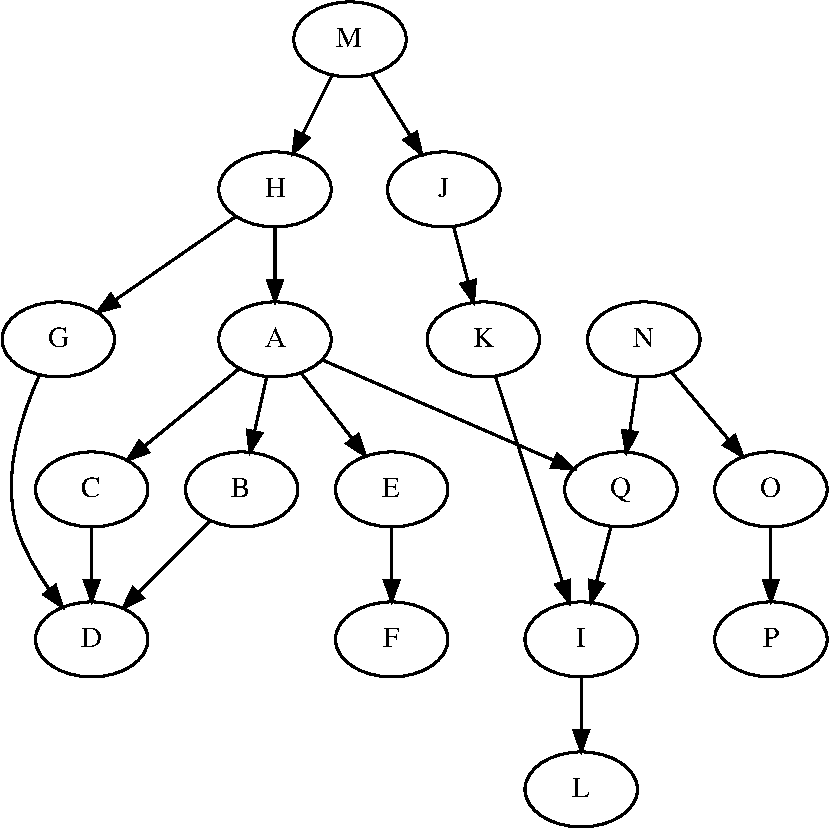
\includegraphics[width=0.3\textwidth]{BermanPlemmons_fig}
\end{center}
If $A\in Z_n$, each of the following conditions is equivalent to the statement ``$A$ is a nonsingular M-matrix''
\end{theorem}
\end{frame}

\begin{frame}
\addtocounter{theorem}{-1}
\begin{theorem}[Continued]
\begin{enumerate}
\item[($A_1$)] All the principal minors of $A$ are positive
\item[($A_2$)] Every real eigenvalue of each principal submatrix of $A$ is positive
\item[($A_3$)] For each $\bx\neq\b0$ there exists a positive diagonal matrix $D$ such that
\[
\bx^TAD\bx>0
\]
\item[($A_4$)] For each $\bx\neq\b0$ there exists a nonnegative diagonal matrix $D$ such that
\[
\bx^TAD\bx>0
\]
\item[($A_5$)] $A$ does not reverse the sign of any vector; that is, if $\bx\neq\b0$ and $\by=A\bx$, then for some subscript $i$, $x_iy_i>0$
\item[($A_6$)] For each signature matrix $S$, there exists an $\bx\gg\b0$ such that
\[
SAS\bx\gg\b0
\]
\end{enumerate}
\end{theorem}
\end{frame}

\begin{frame}
\addtocounter{theorem}{-1}
\begin{theorem}[Continued]
\begin{enumerate}
\item[($B_7$)] The sum of all the $k\times k$ principal minors of $A$ is positive for $k=1,\ldots,n$
\item[($C_8$)] $A$ is nonsingular and all the principal minors of $A$ are nonnegative
\item[($C_9$)] $A$ is nonsingular and every real eigenvalue of each principal submatrix of $A$ is nonnegative
\item[($C_{10}$)] $A$ is nonsingular and $A+D$ is nonsingular for each positive diagonal matrix $D$
\item[($C_{11}$)] $A+D$ is nonsingular for each nonnegative diagonal matrix $D$
\item[($C_{12}$)] $A$ is nonsingular and for each $\bx\neq\b0$ there exists a nonnegative diagonal matrix $D$ such that
\[
\bx^TD\bx\neq 0\quad\textrm{and}\quad \bx^TAD\bx>0
\]
\item[($C_{13}$)] $A$ is nonsingular and if $\bx\neq\b0$ and $\by=A\bx$, then for some subscript $i$, $x_i\neq 0$ and $x_iy_i\geq 0$.
\item[($C_{14}$)] $A$ is nonsingular and for each signature matrix $S$ there exists a vector $\bx>\b0$ such that
\[
SAS\bx\geq\b0
\]
\end{enumerate}
\end{theorem}
\end{frame}

\begin{frame}
\addtocounter{theorem}{-1}
\begin{theorem}[Continued]
\begin{enumerate}
\item[($D_{15}$)] $A+\alpha\II$ is nonsingular for each $\alpha\geq 0$
\item[($D_{16}$)] Every real eigenvalue of $A$ is positive
\item[($E_{17}$)] All the leading principal minors of $A$ are positive
\item[($E_{18}$)] There exists lower and upper triangular matrices $L$ and $U$, respectively, with positive diagonals such that
\[
A=LU
\]
\item[($F_{19}$)] There exists a permutation matrix $P$ such that $PAP^T$ satisfies ($E_{17}$) or ($E_{18}$)
\end{enumerate}
\end{theorem}
\end{frame}

\begin{frame}
\addtocounter{theorem}{-1}
\begin{theorem}[Continued]
\begin{enumerate}
\item[($G_{20}$)] $A$ is \defword{positive stable}; that is, the real part of each eigenvalue of $A$ is positive
\item[($G_{21}$)] There exists a symmetric positive definite matrix $W$ such that
\[
AW+WA^T
\]
is positive definite.
\item[($G_{22}$)] $A+\II$ is nonsingular and
\[
G=(A+\II)^{-1}(A-\II)
\]
is convergent
\end{enumerate}
\end{theorem}
\end{frame}

\begin{frame}
\addtocounter{theorem}{-1}
\begin{theorem}[Continued]
\begin{enumerate}
\item[($G_{23}$)] $A+\II$ is nonsingular and for 
\[
G=(A+\II)^{-1}(A-\II)
\]
there exists a positive definite matrix $W$ such that
\[
W-G^TWG
\]
is positive definite
\end{enumerate}
\end{theorem}
\end{frame}

\begin{frame}
\addtocounter{theorem}{-1}
\begin{theorem}[Continued]
\begin{enumerate}
\item[($H_{24}$)] There exists a positive diagonal matrix $D$ such that 
\[
AD+DA^T
\]
is positive definite
\item[($H_{25}$)] The exists a positive diagonal matrix $E$ such that for $B=E^{-1}AE$, the matrix
\[
(B+B^T)/2
\]
is positive definite
\item[($H_{26}$)] For each positive semidefinite matrix $Q$, the matrix $QA$ has a positive diagonal element
\end{enumerate}
\end{theorem}
\end{frame}

\begin{frame}
\addtocounter{theorem}{-1}
\begin{theorem}[Continued]
\begin{enumerate}
\item[($I_{27}$)] $A$ is \defword{semipositive}; that is, there exists $\bx\gg\b0$ with $A\bx\gg\b0$
\item[($I_{28}$)] There exists $\bx>\b0$ with $A\bx\gg\b0$
\item[($I_{29}$)] There exists a positive diagonal matrix $D$ such that $AD$ has all positive row sums
\item[($J_{30}$)] There exists $\bx\gg\b0$ with $A\bx>\b0$ and
\[
\sum_{j=1}^n a_{ij}x_j>0,\quad i=1,\ldots,n
\]
\item[($K_{31}$)] There exists a permutation matrix $P$ such that $PAP^T$ satisfies ($J_{30}$)
\end{enumerate}
\end{theorem}
\end{frame}

\begin{frame}
\addtocounter{theorem}{-1}
\begin{theorem}[Continued]
\begin{enumerate}
\item[($L_{32}$)] There exists $\bx\gg\b0$ with $\by=A\bx>\b0$ such that if $y_{i_0}=0$, then there exists a sequence of indices $i_1,\ldots,i_r$ with $a_{i_{j-1}i_j}\neq 0$, $j=1,\ldots,r$ and with $y_{i_r}\neq 0$
\item[($L_{33}$)] There exists $\bx\gg\b0$ with $\by=A\bx>\b0$ such that the matrix $\hat A=[\hat a_{ij}]$ defined by
\[
\hat a_{ij} =
\begin{cases}
1 & \text{if } a_{ij}\neq 0\text{ or }y_i\neq 0 \\
0 & \text{otherwise}
\end{cases}
\]
is irreducible
\end{enumerate}
\end{theorem}
\end{frame}

\begin{frame}
\addtocounter{theorem}{-1}
\begin{theorem}[Continued]
\begin{enumerate}
\item[($M_{34}$)] There exists $\bx\gg\b0$ such that for each signature matrix $S$
\[
SAS\bx\gg\b0
\]
\item[($M_{35}$)] $A$ has all positive diagonal elements and there exists a positive diagonal matrix $D$ such that $AD$ is \defword{strictly diagonally dominant}; that is
\[
a_{ii}d_i>\sum_{j\neq i}|a_{ij}d_j|,\qquad i=1,\ldots,n
\]
\item[($M_{36}$)] $A$ has all positive diagonal elements and there exists a positive diagonal matrix $E$ such that $E^{-1}AE$ is strictly diagonally dominant
\end{enumerate}
\end{theorem}
\end{frame}

\begin{frame}
\addtocounter{theorem}{-1}
\begin{theorem}[Continued]
\begin{enumerate}
\item[($M_{37}$)] $A$ has all positive diagonal elements and there exists a positive diagonal matrix $D$ such that $AD$ is \defword{lower semistrictly diagonally dominant}; that is,
\[
a_{ii}d_i\geq\sum_{j\neq i}|a_{ij}d_j|,\qquad i=1,\ldots,n
\]
and
\[
a_{ii}d_i>\sum_{j=1}^{i-1}|a_{ij}d_j|,\qquad i=2,\ldots,n.
\]
\end{enumerate}
\end{theorem}
\end{frame}

\begin{frame}
\addtocounter{theorem}{-1}
\begin{theorem}[Continued]
\begin{enumerate}
\item[($N_{38}$)] $A$ is \defword{inverse-positive}; that is, $A^{-1}$ exists and
\[
A^{-1}\geq 0
\]
\item[($N_{39}$)] $A$ is \defword{monotone}; that is,
\[
Ax\geq 0\Rightarrow x\geq 0\quad\textrm{for all }x\in\IR^n
\]
\item[($N_{40}$)] There exists inverse-positive matrices $B_1$ and $B_2$ such that
\[
B_1\leq A\leq B_2
\]
\item[($N_{41}$)] There exists an inverse-positive matrix $B\geq A$ such that $I-B^{-1}A$ is convergent
\item[($N_{42}$)] There exists an inverse-positive matrix $B\geq A$ and $A$ satisfies ($I_{27}$), ($I_{28}$) and ($I_{29}$)
\end{enumerate}
\end{theorem}
\end{frame}

\begin{frame}
\addtocounter{theorem}{-1}
\begin{theorem}[Continued]
\begin{enumerate}
\item[($N_{43}$)] There exists an inverse-positive matrix $B\geq A$ and a nonsingular M-matrix $C$ such that
\[
A=BC
\]
\item[($N_{44}$)] There exists an inverse-positive matrix $B$ and a nonsingular M-matrix $C$ such that
\[
A=BC
\]
\item[($N_{45}$)] $A$ has a \defword{convergent regular splitting}; that is, $A$ has a representation 
\[
A=M-N,\quad M^{-1}\geq 0,\quad N\geq 0
\]
where $M^{-1}N$ is convergent
\end{enumerate}
\end{theorem}
\end{frame}

\begin{frame}
\addtocounter{theorem}{-1}
\begin{theorem}[Continued]
\begin{enumerate}
\item[($N_{46}$)] $A$ has a \defword{convergent weak regular splitting}; that is, $A$ has a representation
\[
A=M-N,\quad M^{-1}\geq 0,\quad M^{-1}N\geq 0
\]
where $M^{-1}N$ is convergent
\item[($O_{47}$)] Each weak regular splitting of $A$ is convergent
\item[($P_{48}$)] Every regular splitting of $A$ is convergent
\item[($Q_{49}$)] For each $\by\geq\b0$ the set
\[
S_\by=\{\bx\geq\b0: A^T\bx\leq\by\}
\]
is bounded and $A$ is nonsingular
\item[($Q_{50}$)] $S_\b0=\{\b0\}$; that is, the inequalities $A^bx\leq\b0$ and $\bx\geq\b0$ have only the trivial solution $\bx=\b0$ and $A$ is nonsingular
\end{enumerate}
\end{theorem}
\end{frame}


%%%%%%%%%%%%%%%%%%
%%%%%%%%%%%%%%%%%%
%%%%%%%%%%%%%%%%%%
%%%%%%%%%%%%%%%%%%
\begin{frame}[allowframebreaks]
    \frametitle{References}
    \bibliographystyle{amsalpha}
    \bibliography{MATH-4370-7370-lecture-notes.bib}
\end{frame}
    

\end{document}